% !TeX encoding = UTF-8
% !TeX program = xelatex
% !TeX spellcheck = en_US

\documentclass[degree=master,language=english]{thuthesis}
  % 学位 degree:
  %   doctor | master | bachelor | postdoc
  % 学位类型 degree-type:
  %   academic(默认)| professional
  % 语言 language
  %   chinese(默认)| english
  % 字体库 fontset
  %   windows | mac | fandol | ubuntu
  % 建议终版使用 Windows 平台的字体编译


% Initialize
% !TeX root = ./FinalReportCS.tex

% 论文基本信息配置

\thusetup{
  %******************************
  % 注意:
  %   1. 配置里面不要出现空行
  %   2. 不需要的配置信息可以删除
  %   3. 建议先阅读文档中所有关于选项的说明
  %******************************
  %
  % 输出格式
  %   选择打印版(print)或用于提交的电子版(electronic),前者会插入空白页以便直接双面打印
  %
  output = electronic,
  main-language = english,
  language = english,
  %
  % 标题
  %   可使用“\\”命令手动控制换行
  %
  title  = {Final Report of the Guide Study (CS6534)},
  title* = {Final Report of the Guide Study (CS6534)},
  %
  % 学科门类
  %   1. 学术型
  %      - 中文
  %        需注明所属的学科门类,例如:
  %        哲学、经济学、法学、教育学、文学、历史学、理学、工学、农学、医学、
  %        军事学、管理学、艺术学
  %      - 英文
  %        博士:Doctor of Philosophy
  %        硕士:
  %          哲学、文学、历史学、法学、教育学、艺术学门类,公共管理学科
  %          填写“Master of Arts“,其它填写“Master of Science”
  %   2. 专业型
  %      直接填写专业学位的名称,例如:
  %      教育博士、工程硕士等
  %      Doctor of Education, Master of Engineering
  %   3. 本科生不需要填写
  %
  degree-category  = {工学硕士},
  degree-category* = {MsCS},
  %
  % 培养单位
  %   填写所属院系的全名
  %
  department = {计算机科学与技术系},
  %
  % 学科
  %   1. 研究生学术型学位,获得一级学科授权的学科填写一级学科名称,其他填写二级学科名称
  %   2. 本科生填写专业名称,第二学位论文需标注“(第二学位)”
  %
  discipline  = {计算机科学与技术},
  discipline* = {Computer Science},
  %
  % 专业领域
  %   1. 设置专业领域的专业学位类别,填写相应专业领域名称
  %   2. 2019 级及之前工程硕士学位论文,在 `engineering-field` 填写相应工程领域名称
  %   3. 其他专业学位类别的学位论文无需此信息
  %
  % professional-field  = {计算机技术},
  % professional-field* = {Computer Technology},
  %
  % 姓名
  %
  author  = {黄坤伦},
  author* = {HUANG Kunlun},
  %
  % 指导教师
  %   中文姓名和职称之间以英文逗号“,”分开,下同
  %
  supervisor  = {徐, 教授},
  supervisor* = {Professor XU Weitao},
  %
  % 副指导教师
  %
  associate-supervisor  = {陈文光, 教授},
  associate-supervisor* = {Professor Chen Wenguang},
  %
  % 联合指导教师
  %
  % co-supervisor  = {某某某, 教授},
  % co-supervisor* = {Professor Mou Moumou},
  %
  % 日期
  %   使用 ISO 格式;默认为当前时间
  %
  % date = {2019-07-07},
  %
  % 是否在中文封面后的空白页生成书脊(默认 false)
  %
  include-spine = false,
  %
  % 密级和年限
  %   秘密, 机密, 绝密
  %
  % secret-level = {秘密},
  % secret-year  = {10},
  %
  % 博士后专有部分
  %
  % clc                = {分类号},
  % udc                = {UDC},
  % id                 = {编号},
  % discipline-level-1 = {计算机科学与技术},  % 流动站(一级学科)名称
  % discipline-level-2 = {系统结构},          % 专业(二级学科)名称
  % start-date         = {2011-07-01},        % 研究工作起始时间
}

% 载入所需的宏包

% 定理类环境宏包
\usepackage{amsthm}

%\usepackage{amsmath,amsfonts}

\usepackage[bookmarksnumbered, colorlinks, plainpages]{hyperref}

% 也可以使用 ntheorem
% \usepackage[amsmath,thmmarks,hyperref]{ntheorem}

\thusetup{
  %
  % 数学字体
  math-style = TeX,  % GB | ISO | TeX
  math-font  = libertinus,  % stix | xits | libertinus
}

% 可以使用 nomencl 生成符号和缩略语说明
% \usepackage{nomencl}
% \makenomenclature

% 表格加脚注
\usepackage{threeparttable}

% 表格中支持跨行
\usepackage{multirow}

% 固定宽度的表格。
% \usepackage{tabularx}

% 跨页表格
\usepackage{longtable}

% 算法
\usepackage{algorithm}

\usepackage{algpseudocode}

\usepackage{listings}

% 量和单位
\usepackage{siunitx}

% 参考文献使用 BibTeX + natbib 宏包
% 顺序编码制
\usepackage[sort]{natbib}
\bibliographystyle{thuthesis-numeric}

% 著者-出版年制
% \usepackage{natbib}
% \bibliographystyle{thuthesis-author-year}

% 本科生参考文献的著录格式
% \usepackage[sort]{natbib}
% \bibliographystyle{thuthesis-bachelor}

% 参考文献使用 BibLaTeX 宏包
% \usepackage[style=thuthesis-numeric]{biblatex}
% \usepackage[style=thuthesis-author-year]{biblatex}
% \usepackage[style=apa]{biblatex}
% \usepackage[style=mla-new]{biblatex}
% 声明 BibLaTeX 的数据库
% \addbibresource{ref/refs.bib}

% 定义所有的图片文件在 figures 子目录下
\graphicspath{{figures/}}

% 数学命令
\makeatletter
\newcommand\dif{%  % 微分符号
  \mathop{}\!%
  \ifthu@math@style@TeX
    d%
  \else
    \mathrm{d}%
  \fi
}
\makeatother

% hyperref 宏包在最后调用
\usepackage{hyperref}


\thusetup{
toc-chapter-style = times,
}
\thusetup{
  cite-style = inline,
}

\begin{document}


% Frontend
\maketitle


\frontmatter
%\input{data/abstract}

% Menu
\tableofcontents

% Figures and appdiex
% \listoffiguresandtables  % 插图和附表清单(仅限研究生)
%\listoffigures           % 插图清单
%\listoftables            % 附表清单

% 符号对照表
%\input{data/denotation}


% Main Articles
\mainmatter
% !TeX root = ../FinalRepordCS.tex

\chapter{Introduction}

\section{Background}

Network security is a recent scorching topic and affects everyone's vital interests. Mature PKI-based password management systems such as SSL and TLS are regarded as an excellent way to solve the problem of encrypted communication in computer networks. However, in the field of the Internet of Things, due to issues such as node computing performance and the difficulties in key management in large amount of nodes, PKI systems are not suitable in it. 

According to Gartner\cite{gartnerresearchiot}, there will be over 43 billion IoT devices connected to the internet by 2023, and the IoT market size will reach US\$1.4 trillion. The rapid development of the IoT is mainly due to the following trends. Also, the MIIT suggests that the IoT is a future development trend that will have a profound impact on all industries\cite{iot13th5yr}. The security of the communication channel in the Internet of Things is of utmost importance, given the critical role of IoT. Ensuring the security of IoT communication channels will be a highly significant and crucial subject.

To address this problem, and based on previous research, some physical layer key generation methods have been proposed. Physical layer key generation is a technique for generating cryptographic keys from the physical characteristics of a wireless communication channel. This can be done by exploiting the unique features of the channel, such as its fading characteristics, noise properties, and path loss. Physical layer key generation is particularly attractive for wireless sensor networks (WSNs) because it does not require any prior shared information between the nodes, and it can be implemented with relatively low computational overhead.

Physical layer key generation has recently been a research hotspot in academia and industry\cite{7120014}. However, existing research often focuses only on traditional wireless communication technologies such as Wi-Fi, ZigBee, and 5G Radio Access Network. However, in the area of Low-Power Wide-Area Networks (LPWAN)\cite{iotfactorylpwan}, the long communication distance, low power consumption, and low transmission rate bring new research challenges to physical layer key generation.
\begin{figure}
  \centering
  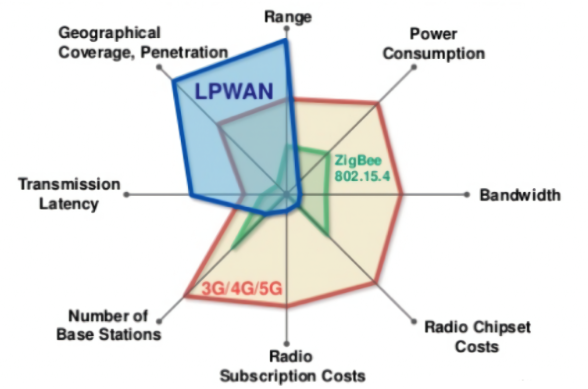
\includegraphics[width=0.6\linewidth]{fig1-1.png}
  \caption{LPWAN vs. Other wireless communication technologies\cite{iotfactorylpwan}}
  \label{fig:1-1}
\end{figure}
LoRa, a widely used LPWAN communication technology, is a physical layer modulation method defined by Semtech Corporation and based on the Chirp spread spectrum technology, which achieves a reception sensitivity of -148 dBm, a small data rate (0.3-50kbps) in exchange for a high communication range (3km in urban areas and 15km in suburban areas) and low power consumption (battery-powered operation for up to 10 years under certain conditions)\cite{lorawanpara}. It provides a reliable connectivity solution for low-power IoT devices, especially for communication or data interaction with outdoor wireless sensor networks.
\begin{figure}
  \centering
  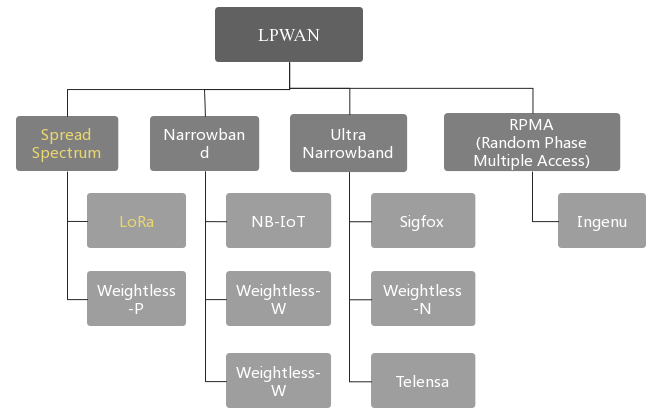
\includegraphics[width=0.8\linewidth]{fig1-2.png}
  \caption{LPWAN Classification}
  \label{fig:1-2}
\end{figure}
Despite many advantages, the biggest problem is that physical layer encryption for LoRa is not well standardized. Because it is a type of wireless communication tech that has to broadcast its signal, it makes the communication information easy to capture and monitor. Thus, physical layer encryption for LoRa communication is a significant topic. 

In short, physical layer key generation for LoRa is still under development, but it can potentially revolutionize the security of LoRa-based networks. It can be used to secure a wide range of applications, including smart cities, industrial automation, and the Internet of Things.

\section{Objectives}

The specific research objectives are:

1. Understand the characteristics and limitations of LoRa communication technology, including its communication range, power consumption, data rate, and noise immunity.

2. Select and configure suitable LoRa modules and development boards to realize the LoRa communication protocol stack and basic data transmission functions.

3. Implement a physical layer encryption algorithm for LoRa communication to protect the privacy and confidentiality of data. The algorithm should suit LoRa's low data rate and long communication distance characteristics and have strong anti-interference and anti-jamming capabilities.

4. Test and evaluate the performance of the encryption algorithm via multiple scenario experiments and simulations. Compare the performance with existing key generation algorithms for LoRa physical layer and analyze its pros and cons.


% !TeX root = ../FinalRepordCS.tex

\chapter{Related Work}
According to the previous research, some methods of key generation based on the physical layer of the LoRa communication protocol were proposed. However, Physical layer key generation for LoRa is still under development, but it has the potential to revolutionize the security of LoRa-based networks. It can be used to secure a wide range of applications, including smart cities, industrial automation, and the Internet of Things.
Physical layer key generation for LoRa is a promising technique for establishing secure communication links in LoRa-based networks. Physical layer key generation exploits the randomness and reciprocity of the LoRa channel to extract a secret key shared by the communicating devices. This key can then be used to encrypt and decrypt their communication, ensuring confidentiality and integrity.

\section{Theoretical Foundations}

\subsection{Physical Layer Key Generation}
Physical layer key generation is the way to generate a shared secret key between wireless devices by exploiting the reciprocity of the random fading channel, in which wireless devices measure highly correlated wireless channel characteristics (e.g., channel impulse responses or received signal strengths) and use them as shared random sources to generate a shared key. In theory, in a rich multipath scattering environment, a passive attacker who is more than a half-wavelength away from the legitimate users will obtain uncorrelated channel measurements and thus cannot infer much information about the generated key. The physical layer key generation mechanisms do not require expensive computation and have the potential to achieve information-theoretic security in the sense that the secrecy of the generated key is not dependent on the hardness of a computational problem but relies on the physical laws of the wireless fading channels.[3] 
Generally, physical layer key generation applies the following five steps to generate a key: channel probing, randomness extraction, quantization, information reconciliation, and privacy amplification, illustrated in Figure 2.1.
\begin{figure}
  \centering
  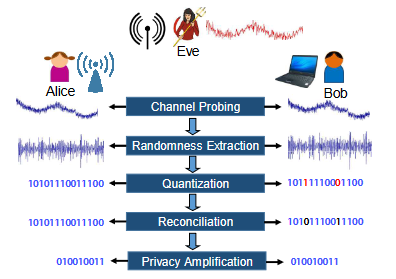
\includegraphics[width=0.6\linewidth]{fig2-1.png}
  \caption{Secret key generation model[3]}
  \label{fig:2-1}
\end{figure}

\subsection{LoRa Physical Layer Protocol}
LoRa adopts the Chirp Spread Spectrum (CSS) modulation mechanism, which provides anti-interference and long-range communication capability. As shown in Figure 2.2(a) and (b), a base symbol in LoRa physical layer protocol (PHY) is a chirp with frequency linearly increasing with time. The start frequency (fstart ) of a symbol represents the encoded information. A LoRa symbol has two segments with a sharp frequency drop, as shown in Figure 2-2(c).
\begin{figure}
  \centering
  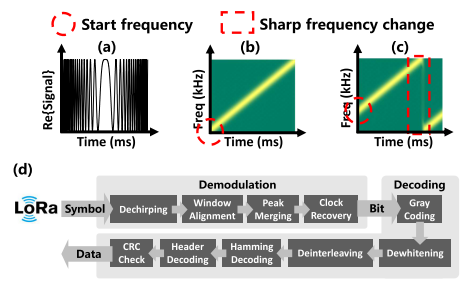
\includegraphics[width=0.7\linewidth]{fig2-2.png}
  \caption{(a) Real part of a base up-chirp symbol. (b) Base up-chirp symbol. (c) Shifted symbol. (d) Complete procedure of LoRa PHY\cite{10.1145/3546869}}
  \label{fig:2-2}
\end{figure}
And the RSSI (Received Signal Strength Indicator) is a relative measurement that helps us determine if the received signal is strong enough to get a good wireless connection from the transmitter. Since LoR supports bi-directional communication, The RSSI is an important measurement for both gateways and end devices. And RSSI is measured in dBm and its value is a negative form. The closer the RSSI value is to zero, the received signal is stronger, the good examples for positive and negative have shown in Figure 2.3 (a) and (b)\cite{rssiandsnrfigure}. And the following factors mainly influence the RSSI: Path loss, Antenna gain, Cable/connector loss.
\begin{figure}
  \centering
  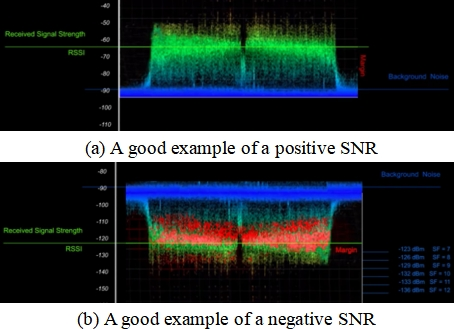
\includegraphics[width=0.6\linewidth]{fig2-3.png}
  \caption{example of a positive/negative SNR}
  \label{fig:2-3}
\end{figure}

\section{Existing Solutions}
\subsection{CFR-Based Physical Layer Key Generation}
One common approach to Physical layer key generation for LoRa is to use the fine-grained channel frequency response (CFR). Y. Peng et al. proposed a secret key generation method from CFR for OFDM TDD systems\cite{7054386}. Moreover, H. Luo et al. proposed a Channel Frequency Response-Based Secret Key Generation Scheme in In-Band Full-Duplex MIMO-OFDM Systems\cite{10158732}. When receiving \(I_{MS}\), both BS and MS construct a CFR estimate vector at the agreed subcarrier index set \(I_{MS}\) as
\begin{equation} 
  \hat{H}_{U}(I_{MS})   = \left [ \hat{H}_{U}(f_{(1)})\hat{H}_{U}(f_{(2)}) ...\hat{H}_{U}(f_{1(T_{b})}) \right ], where\ u\in \left \{ BS, MS  \right \}   
\end{equation} 
and then generate the secret key
\begin{equation} 
  K_{U}  = \left [ K_{U}({(1)})K_{U}{(2)} ...K_{U}({2T_{b}}) \right ]
\end{equation} 

The CFR is an unique characteristic of the LoRa channel that depends on the distance, orientation, and other environmental factors. By estimating the CFR at both ends of the communication link, the devices can generate a secret key that is shared only between them.
\subsection{RSSI-Based Physical Layer Key Generation}
Another approach to physical layer key generation for LoRa is to use the received signal strength indicator (RSSI). The RSSI is a measure of the strength of the received signal. S. Jana et al. evaluated the effectiveness of secret key extraction for private communication between two wireless devices from the received signal strength variations on the wireless channel between the two devices\cite{10.1145/1614320.1614356}. After that, W. Xu et al. employed a number of signal processing techniques to improve key generation rate significantly and proposed a novel compressive sensing-based reconciliation framework to reduce the mismatch rate\cite{8580375}. 
\begin{equation} y = y_{\mathrm{ Bob}}-y_{\mathrm{ Alice}}= A \left ({K_{\mathrm{ Bob}}-K_{\mathrm{ Alice}}}\right) + e= A x +e \end{equation} 
\begin{equation} \mathop {\mathrm {arg\,min}} _{x} \| x \|_{1} \quad \text {subject to}~ ~\left \|{y - Ax}\right \|_{2} < \epsilon.\end{equation} 
\begin{equation}K_{\mathrm{ Alice}}^{'} = K_{\mathrm{ Alice}} \oplus x\end{equation} 

The RSSI is also affected by the distance and other environmental factors. By exchanging RSSI measurements, the devices can generate a secret key that is shared only between them.

\subsection{Chaos-based Physical Layer Key Generation}
One another emerging technique for physical layer key generation in wireless networks is the use of chaos theory. The chaotic behavior of the wireless channel can be exploited to generate a random bit sequence that is used as a secret key shared only between the communicating devices. Yahya M. Al-Moliki et al. proposed a chaotic key creation approach, that is introduced by including the position-sensitive and real-valued channel state information of the VLC channel\cite{https://doi.org/10.1049/iet-opt.2018.5072}. 
\begin{equation}{\widehat {\mathbf{s}}_k} = \arg \mathop {\min }\limits_{{\mathbf{s}}_k^{(i)} \in {\mathbf{S}}} {\left\| {{{\mathbf{r}}^{(k)}} - {h_k}{\mathbf{s}}_k^{(i)}} \right\|^2};k = 1, \ldots ,K\end{equation}
where
\begin{equation}{{\mathbf{r}}^{(k)}} = \begin{cases} {\mathbf{r}}&{;{\text{ for }}k = 1} \\ {{{\mathbf{r}}^{(k - 1)}} - {h_{k - 1}}{{\widehat {\mathbf{s}}}_{k - 1}}}&{;{\text{ for }}k = 2, \ldots ,K.} \end{cases}\end{equation}
then, the output of the \(k^{th}\) stage is demodulated as \({{\hat{\mathbf b}}_k} = \left[ {\begin{array}{lll} {{{\hat b}_{k,1}}}& \ldots &{{{\hat b}_{k,U}}} \end{array}} \right]\).
The chaotic nature of the wireless channel ensures that the generated key is random and difficult to predict, making it difficult for adversaries to eavesdrop on the communication link.
\subsection{Deep-Learning-Based Physical Layer Key Generation}
A related approach to physical layer key generation for wireless network is the use of machine learning algorithms. Deep learning or machine learning algorithms can be used to analyze the wireless channel characteristics and identify patterns that can be used to generate a secret key. For example, by using supervised learning algorithms, the devices can analyze the wireless channel behavior and identify features that are unique to each communication link. These features can then be used to generate a unique secret key that is shared only between the devices. X. Zhang et al. implemented a Deep-Learning-Based Physical-Layer Secret Key Generation for FDD Systems using the adaptive moment estimation (ADAM) algorithm with the following loss function\cite{9526766}. 
\begin{equation} {\mathrm{ Loss}}_{\mathbb {D}}\left ({\boldsymbol {\Omega }}\right) = {\mathrm{ MSE}}\left ({\widehat {\mathbf {x}}_{2}, \mathbf {x}_{2}}\right)=\frac {1}{VN_{\mathbf {x}}}\sum _{v=0}^{V-1}\left \|{\widehat {\mathbf {x}}_{2}^{\left ({v}\right)} -\mathbf {x}_{2}^{\left ({v}\right)}}\right \|_{2}^{2}\end{equation} 
\subsection{Quantum-Based Physical Layer Key Distribution}
Using quantum mechanics principles for physical layer key distribution is also a promising approach for wireless networks. Quantum mechanics principles can be applied to generate truly random keys using the quantum states of particles. The devices can use quantum states of particles to generate random bits that are used as secret keys for encrypting and decrypting their communication. Using quantum keys ensures that the key is truly random and cannot be predicted or intercepted by an adversary. However, several technical limitations, such as channel losses and transmission distance, should be overcome before it comes to practical application.

\section{Advantages and Disadvantages}
Firstly, chaos theory for physical layer key generation in wireless networks has several strengths and weaknesses. On the one hand, the chaotic behavior of the wireless channel ensures that the generated key is random and difficult to predict, making it difficult for adversaries to eavesdrop on the communication link. This approach provides high security and randomness, which is essential for secure communication. However, on the other hand, using chaos theory for physical layer key generation may be challenging in practical implementation. The chaotic behavior of the wireless channel may be difficult to characterize and control in practical environments, making it difficult to ensure consistent and reliable key generation. Also, chaos theory may be more complex mathematical than other key generation techniques, making it challenging to implement and scale in resource-constrained environments.

Secondly, using quantum-based principles for physical layer key distribution in wireless networks has several strengths and weaknesses. On the one hand, quantum keys ensure that the key is truly random and cannot be predicted or intercepted by an adversary, providing high security and randomness. This approach is auspicious for ensuring secure communication in wireless networks. However, on the other hand, the quantum-based is typically designed for optical fiber or free-space optical communication, not for RF wireless communication like LoRa. The use of quantum mechanics principles may be challenging in practical implementation. Generating quantum keys requires using specialized quantum devices and technologies that may not be widely available or practical for resource-constrained environments. Additionally, quantum communication is weaker to practical imperfections than classical communication, making it difficult to ensure consistent and reliable key distribution under practical conditions. 

Thirdly, the Deep-learning-based method offers promising security and key establishment advantages without pre-shared secrets. However, it also faces challenges related to data quality, model vulnerabilities, and resource constraints. It is not a standard or suitable choice for LoRa technology due to resource constraints, data availability, real-time requirements, complexity, and the presence of established security measures within the LoR protocol. Implementing Deep-Learning-Based LoRa networks would require overcoming these challenges and aligning with the specific requirements and limitations of LoRa technology.

Such three methods fundamentally differ in operating principles, resource requirements, environmental sensitivity, standardization, and security considerations. Typically, the hardware performance of LoRa nodes, including the CPU and memory specifications limitation, is designed for Low-Power and Battery-Operated, which means they are not providing such calculation performance.

Thus, no matter in theory or industrial area, most research on the Physical-Layer Secret Key Generation for LoRa are based on their wireless channel characteristics as very fast and efficient to implement in LoRa Node.

\section{Relationship with Proposed Solution}
In the context of the guide study, the primary focus revolves around the inherent characteristics of the Internet of Things. Given the inherent constraints imposed by the limited computational capacity of LoRa nodes and a spectrum of attributes, including communication speed and error rates, I have elected to adopt a widely acknowledged approach within the industry. This approach, rooted in the Received Signal Strength Indicator principles, serves as the foundation for the generation of physical-layer cryptographic keys. Moreover, my methodology draws inspiration from established practices documented in pertinent literature. To enhance the quality of the raw signal data, I intend to implement a series of preprocessing techniques, encompassing bit quantization and signal demodulation.

The present study and research direction exhibit significant potential, particularly within the realm of the Internet of Things and the nuanced field of physical-layer key generation facilitated by LoRa technology. 

Preprocessing Methodologies: In the context of managing RSSI data, the employment of advanced preprocessing techniques assumes paramount importance. Strategies such as bit quantization and signal demodulation should be explored in depth, and their application should be calibrated to optimize precision and accuracy.

An inclusive and thorough approach to validation should be adopted, spanning a spectrum of operational contexts that encapsulate the diversity of real-world IoT deployment scenarios. Rigorous validation across an array of settings, encompassing both indoor and outdoor environments, as well as scenarios with varying degrees of obstruction, will ensure the adaptability and efficacy of the proposed method.

Furthermore, I have meticulously devised a comprehensive validation strategy tailored to the real-world deployment scenarios characteristic of LoRa technology. The testing plan includes but is not limited to the potential critical use case for LoRa technology, which is in the field of environmental monitoring. By doing so, I endeavor to substantiate the practical applicability of the theoretical framework I have laid out. Also, the methodical planning and meticulous experimental design are the cornerstones of empirical validation. The experimental framework should be meticulously devised to yield a substantial corpus of empirical evidence, reflecting the manifold operational contexts under scrutiny.

% !TeX root = ../FinalRepordCS.tex

\chapter{Project Outline and Methodology}

\section{Project Overview}
In this project, I am supposed to mainly implement each LoRa node hardware with a programmable Arduino shield and a Dragino’s LoRa expansion board for Arduino and then program the communication protocol with the Arduino IDE software with the LoRa KIT. Including the following:
The implementation of LoRa nodes’ communication, such as signal sending and receiving, coding and decoding,
The extraction and analysis of the physical layer information between the communication process,
The implementation of the LoRa key generation and the test on it.
For the current interim progress, I have already implemented the following:

1.LoRa Physical Protocol emulation,

2.The design of each programmable Arduino shield for LoRa communication,

3.The logical implement of the programmable shields for LoRa,

4.Deep-in-Building Test Data Collection.

\section{Methodology}

\subsection{LoRa Physical Layer Emulation and Analyst}
Before the design and development in real vibe, the understanding and simulation of the LoRa physical layer could be significant since it has its characteristic, which is different from the standard communication protocol.
The LoRaPHY KIT is for LoRa Physical Protocol emulation\cite{10.1145/3546869}. Through this KIT, the payload of LoRa can be simulated, especially, and the encryption information can be analyzed and visualized before and after.
\begin{figure}
  \centering
  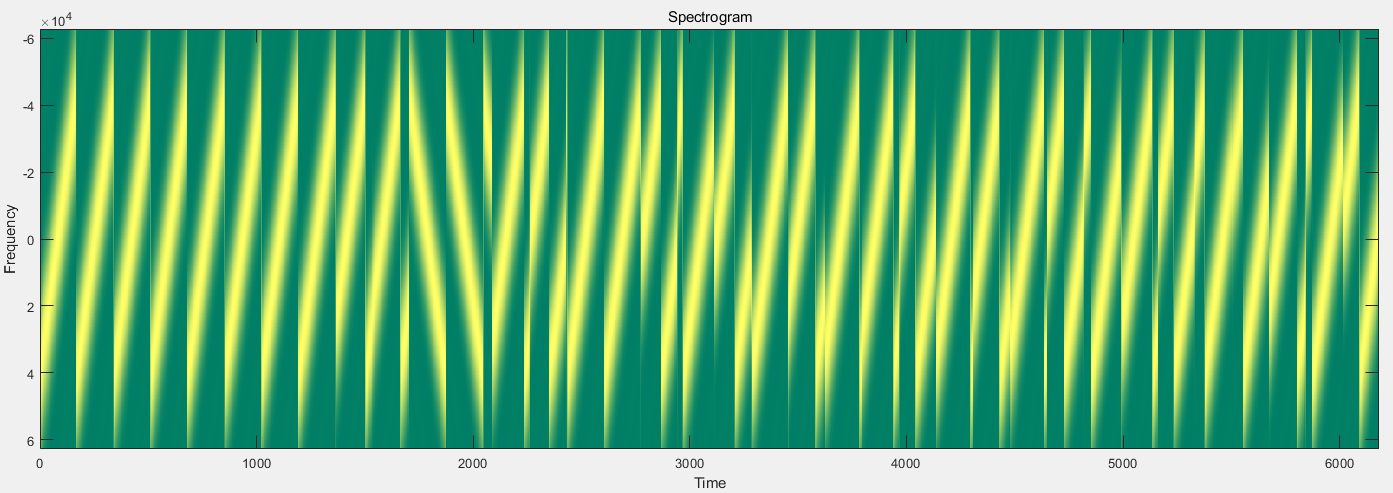
\includegraphics[width=1\linewidth]{fig3-1.png}
  \caption{A emulated LoRa physical layer payload of ‘[78 22 43 44 12]’}
  \label{fig:3-1}
\end{figure}

\subsection{Arduino Shield featuring LoRa technology}
Typically, LoRa uses SX127x chipset, as shown as Fig 3-2, by Semtech, and an Arduino Shield features LoRa technology based on an Open source library. This shield allows users to send data and reach extremely long ranges at low data rates. It provides ultra-long-range spread spectrum communication and high interference immunity while minimizing current consumption. It is on the Semtech SX1276/SX1278 chip, and it targets professional wireless sensor network applications such as irrigation systems, smart metering, smart cities, and building automation.
Moreover, using the SX127x LoRa technique, the shield can achieve a sensitivity of over -148dBm using a low-cost crystal and bill of materials. The high sensitivity combined with the integrated +20 dBm power amplifier yields an industry-leading link budget, making it optimal for any application requiring range or robustness.
By using these components, the LoRa communication protocol can be well physically implemented and is a powerful and adaptable tool that can support the realization of the project.
\begin{figure}
  \centering
  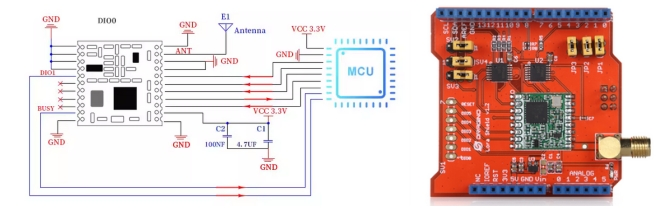
\includegraphics[width=1\linewidth]{fig3-2.png}
  \caption{The SX127x schematic diagram and physical representation}
  \label{fig:3-2}
\end{figure}

\subsection{Arduino’s UNO Programmable Board and IDE}
The Arduino Uno is a popular microcontroller board widely used in the maker and electronics communities for various projects and prototypes. Although the Arduino Uno itself does not possess native LoRa capabilities, it can be effectively employed as a control and interface unit to facilitate seamless integration with external LoRa modules or chipsets, shown as Fig 3-4. The integration process entails meticulous wiring connections between the Arduino Uno and the LoRa module, encompassing essential pins such as those for power (3.3V or 5V), ground (GND), and serial communication (TX and RX). Voltage levels are diligently considered to ensure compatibility between the Arduino Uno and the LoRa module. 
\begin{figure}
  \centering
  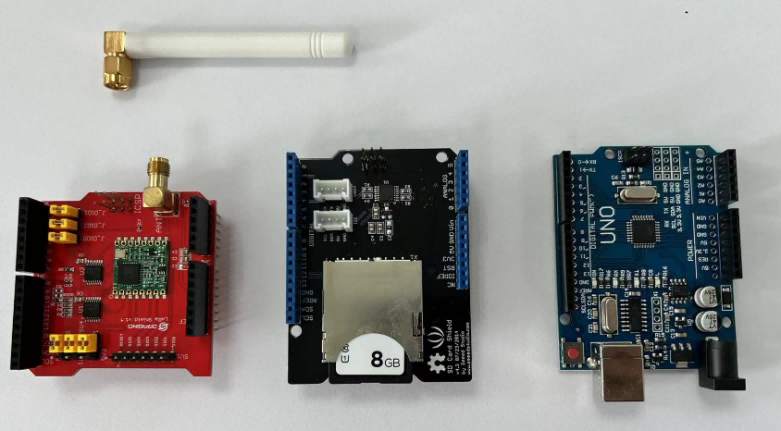
\includegraphics[width=0.6\linewidth]{fig3-3.png}
  \caption{The SX127x and Arduino’s UNO Programmable Board}
  \label{fig:3-3}
\end{figure}
In addition to the essential connections, supplementary connections, such as those related to module reset or configuration, may be required depending on the module's specifications. To facilitate effective communication with the LoRa module, the Arduino IDE is utilized. Relevant libraries that optimize interactions with the LoRa module are installed, ensuring the Arduino Uno is aligned with the specific requirements of the chosen module.
The subsequent phase entails the creation of Arduino code tailored to configure and orchestrate communication with the LoRa module. This code encompasses fundamental tasks such as module initialization, parameter configuration (e.g., frequency, spreading factor, bandwidth), and the transmission or reception of LoRa data packets. The intricacies of the code are contingent upon the precise LoRa module chosen and the intended application. Upon the completion of the code development, it is compiled and uploaded to the Arduino Uno via the ubiquitous USB interface, positioning the controller as a command and control center for the LoRa module.
By using this set of components, it is possible to effectively implement the logic for sending and receiving data between various LoRa nodes, as well as extracting features such as RSSI from the communication channel. Additionally, it enables the implementation of logic for physical layer encryption.


\subsection{Deep-in-Building and Outdoor Test}
The comprehensive evaluation of LoRa communication systems necessitates the execution of rigorous deep-in-building and outdoor tests, each designed to address distinct aspects of performance and coverage within varying environmental contexts.
The principal objective of the deep-in-building test for LoRa communication is to scrutinize the signal propagation characteristics within the intricate confines of interior structures, encompassing walls, floors, and architectural elements.
The outdoor test regimen for LoRa communication entails a meticulous assessment of the system's performance attributes in open-air or outdoor settings, characterized by the absence of indoor obstructions.
\begin{figure}
  \centering
  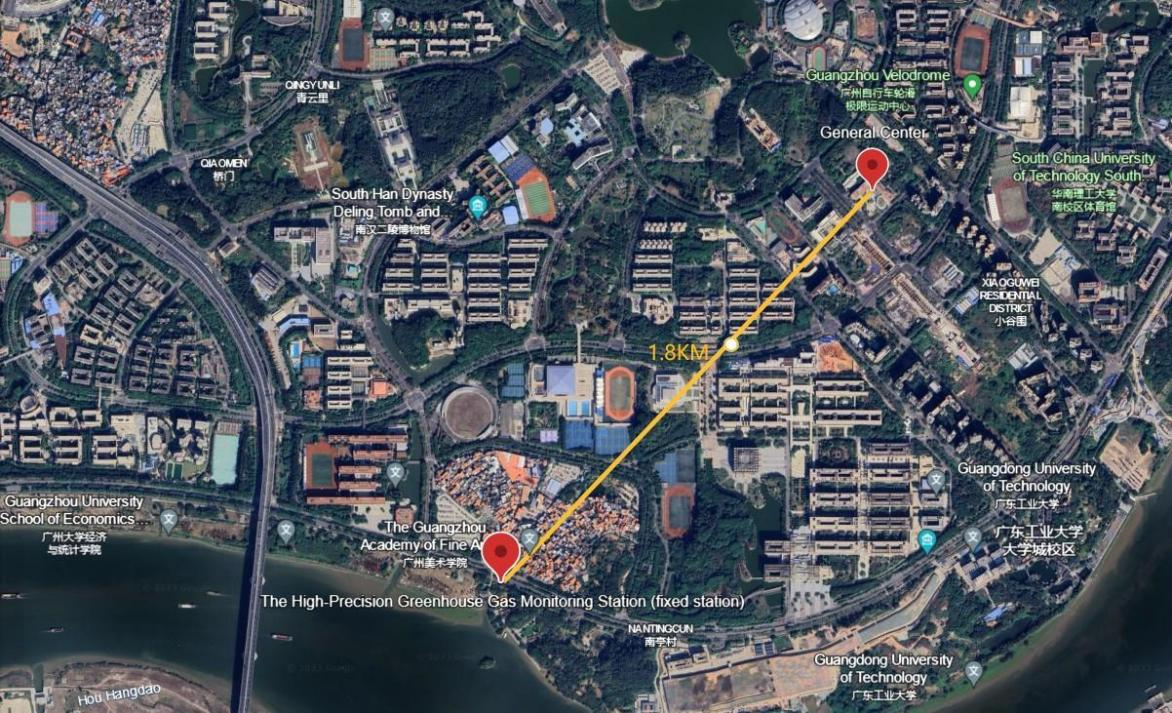
\includegraphics[width=1\linewidth]{fig3-4.png}
  \caption{Outdoor test between an fixed High-Precision Greenhouse Gas Monitoring Station and the General Center (1.8km)}
  \label{fig:3-4}
\end{figure}
At the same time, this testing plan is combined with a potential critical use case for LoRa technology in the field of environmental monitoring\cite{8515030}. Currently, most environmental monitoring data is transmitted using mobile networks, which can be costly and dependent on the infrastructure of telecommunication operators. In remote areas like the wilderness or deep in the mountains, there is often a lack of cellular signal coverage, even though environmental monitoring activities frequently need to be conducted in these areas. Therefore, this testing plan encompasses outdoor fixed monitoring stations, central monitoring facilities, and mobile monitoring stations for environmental monitoring. It is expected to effectively carry out a series of tests, including deep-in-building and outdoor tests.
\begin{figure}
  \centering
  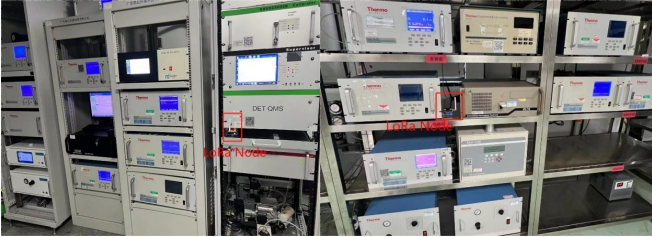
\includegraphics[width=1\linewidth]{fig3-5.png}
  \caption{Deep-In-Building Test at General Center}
  \label{fig:3-5}
\end{figure}

\subsection{Data Extraction and Analyst}
By testing in various scenarios, a series of test data can be obtained. The next step is to extract and preprocess the data. In particular, the analysis of feature data from the signals. Through the analysis of this data, we can understand the characteristics of LoRa signal features in different scenarios and under different electromagnetic background interferences.
Also, the Savitzky-Golay filter will be applied to the raw signal datasets. The filter is a commonly used technique in signal processing for smoothing or filtering noisy data, especially in the field of spectroscopy and chromatography. The primary goal of the Savitzky-Golay filter\cite{doi:10.1021/ac60214a047} is to remove noise from a signal while preserving the important features, such as peaks and valleys. It works by fitting a polynomial to a small window of data points and then using this polynomial to estimate the value of the central data point. This process is repeated for all data points, effectively smoothing the signal.
\begin{figure}
  \centering
  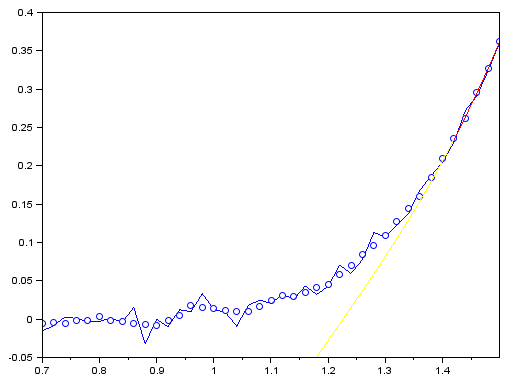
\includegraphics[width=0.5\linewidth]{fig3-6.png}
  \caption{Savitzky-Golay filter}
  \label{fig:3-6}
\end{figure}
After the data extraction and preprocessing, the analyst can begin to explore the characteristics of LoRa signal features in different scenarios and under different electromagnetic background interferences. This analysis will help to determine the optimal communication parameters and signal processing methods for specific applications. And Based on the results of these tests, the analyst can provide decision-makers with data-driven insights on how to optimize LoRa communication systems for different environmental contexts. This information is crucial for companies and organizations to make informed decisions about how to design, deploy, and maintain LoRa communication networks that are reliable and efficient for their specific applications.

\subsection{Physical Key Generation}
Physical layer key generation is a method for generating a shared secret key between wireless devices by exploiting the reciprocity of the random fading channel. And wireless devices measure highly correlated wireless channel characteristics and use them as shared random sources to generate a shared key.
In this section, the primary focus is on the physical layer key generation based on relevant algorithms. This includes the processing of signal feature data using methods such as Bit-Quantization and reconciliation. Additionally, it involves comparing the key matching rates and key generation speeds for different parameters values. Some related research achievements in Lora physical layer encryption will be utilized in this chapter.

\subsection{Attempt on Decentralization of Key Distribution}
After testing the physical layer key generation algorithms, considering the communication characteristics of IoT and the limited memory and computational capabilities of LoRa nodes, an attempt will be made to propose a decentralized physical layer generation scheme based on node calculations.
% !TeX root = ../FinalRepordCS.tex

\chapter{System modeling and structure}

\section{Communication Architecture}

The architecture mainly describes Alice and Bob as two LoRa nodes that need to generate the same communication key. It starts with one of them initiating the key generation communication (a random LoRa message with a sequence number). When the other party (Bob) receives the request, it immediately replies with a message with a sequence number.

The pair of two LoRa packets that in the communicate with each other are both marked with RSSI. These tags are mainly generated by the strength of the signal via the communication. Since wireless message transmission can be regarded as extremely fast propagation, which is close to the speed of light, the RSSI values that the two nodes can obtain in this communication process are close. Or, to be more specific, if LoRa messages are generated with the same pattern, the trend of RSSI values obtained at both ends over a period of time is close.
In addition, since RSSI is mainly affected by signal strength, in the real world, it is generally due to changes in the surrounding environment, such as changes in the communication distance between the two nodes, the appearance of some obstacles between the nodes, the weather, or interference from other signals, etc. For the two nodes, the impact is the same, especially for the physical communication channel formed by the two nodes. Therefore, the trend of RSSI values obtained by the two nodes is a good physical layer feature factor.
\begin{figure}
  \centering
  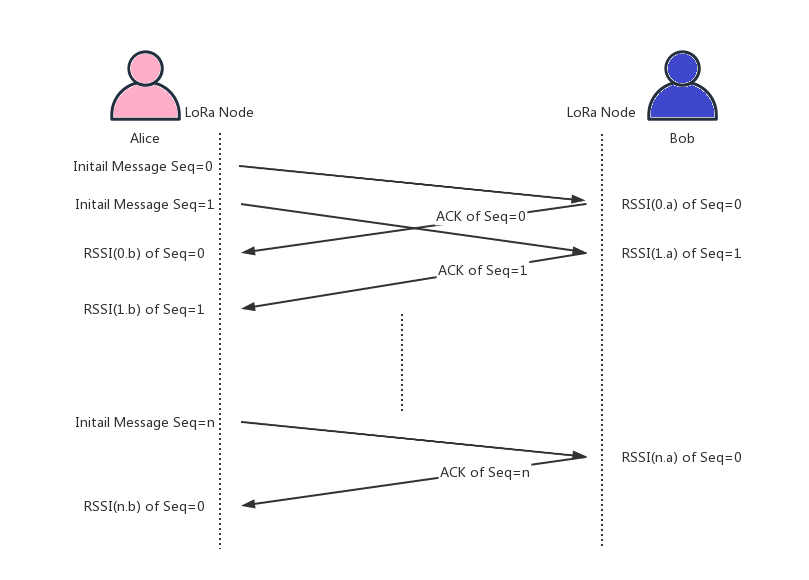
\includegraphics[width=0.7\linewidth]{fig4-1.png}
  \caption{Communication Architecture}
  \label{fig:4-1}
\end{figure}
As shown in the figure \ref{fig:4-1}, after \(n\) interactions, \(n\) pairs of RSSI values can be obtained. Then, through a certain algorithm, the \(n\) pairs of RSSI values can be modulated and used as factors to generate a key. In this way, the two nodes can obtain a common physical layer communication key. 
However, in actual use, due to interference from the actual environment, such as physical obstruction, channel blocking, and frequency band interference, the LoRa communication packets cannot always be received as expected. In particular, due to long-distance transmission, LoRa physical layer messages are not reliable transmissions, so packet loss needs to be considered. In addition, according to this communication model, the biggest challenge to generating a pair of RSSI is still Bob's reply message. This is because Bob's reply is based on the premise of receiving Alice's message, but Alice may not be able to receive Bob's reply.
\section{LoRa End Nodes Modeling and Algorithm}
As mentioned in the previous text, LoRa nodes are half-duplex devices. In order to implement the mentioned functional model, a specific algorithm is required to enable LoRa nodes to both listen to messages and transmit messages after receiving information.

One way to implement this functional model is to use a polling approach. In this approach, LoRa nodes periodically poll other nodes to see if they have any information to send. If the polling detects that other nodes have information to send, the LoRa node will stop listening and transmit a message.Another way to implement this functional model is to use an event-driven approach. In this approach, LoRa nodes register an event handler that will be triggered when they receive information from other nodes. When the event handler is triggered, the LoRa node will stop listening and transmit a message.

Specifically, in the polling approach, LoRa nodes can use the following steps to implement the aforementioned functional model:
\begin{itemize}
  \item Set a polling interval, such as 100 milliseconds.
  \item Within the polling interval, LoRa nodes will send a query message to other nodes.
\end{itemize}

In the event-driven approach, LoRa nodes can use the following steps to implement the aforementioned functional model:
\begin{itemize}
  \item Register an event handler that will be triggered when they receive information from other nodes.
  \item In the event handler, LoRa nodes will stop listening and transmit a message.
\end{itemize}

Both of these algorithms have their own advantages and disadvantages. The advantage of the polling approach is that it is simple to implement, but it can reduce the LoRa node's receiving sensitivity. The advantage of the event-driven approach is that it can improve the LoRa node's receiving sensitivity, but it requires additional overhead for the event handler.
\begin{algorithm}[hbt!]
  \caption{Algorithm for Alice}\label{alg:Alice}
  \begin{algorithmic}
  \State Initialize variables:
      \State $lastSendTime \gets 0$
      \State $interval \gets$ user-defined interval
      
      \Function{loop}{}
          \If{$\text{millis()} - \text{lastSendTime} > \text{interval}$}
              \State $message \gets \text{``SEQ"} \gets n$
              \State \Call{sendMessage}{$message$}
              \State \textbf{print} ``Sending" $+$ $message$
              \State $lastSendTime \gets \text{millis()}$
              \State $interval \gets \text{random}(2000) + 1000$ \Comment{2-3 seconds}
          \EndIf
          \State \textbf{parse for a packet, and call} \Call{onReceive}{\text{parsePacket()}}
      \EndFunction
  \end{algorithmic}
\end{algorithm}
The purpose of this algorithm is to establish a two-way communication channel over LoRa. The “SEQ” message is a special message that is used to initiate a communication session. The onReceive() function can be used to process any incoming messages, such as acknowledgment messages or data messages.
The loop starts by checking the millis() function to see how long it has been since the last message was sent. If it has been longer than the interval period, then the loop sends a SYN message using the sendMessage() function.
The loop then calls the onReceive() function to parse for any incoming packets. If a packet is received, the onReceive() function will be called with the parsed packet data.
\begin{algorithm}[hbt!]
  \caption{Algorithm for sendMessage}\label{alg:sendMessage}
  \begin{algorithmic}
  \Function{sendMessage}{$\text{outgoing}$}
          \State Initialize $message$
          \State Add $message \gets \text{Payload} \gets outgoing$
          \State Send $message$
          \State $msgCount \gets$ $msgCount + 1$
      \EndFunction
  \end{algorithmic}
  \end{algorithm}
The sendMessage algorithm encapsulates a message for LoRa communication. It constructs a packet containing destination and sender addresses, a message ID, payload length, and the actual message. The LoRa packet is then sent, and the message ID is incremented for the next message. This function is designed for a larger program implementing LoRa communication.
  \begin{algorithm}[hbt!]
    \caption{onReceive Algorithm for Alice}\label{alg:onReceive}
    \begin{algorithmic}
        \Function{onReceive}{$\text{packetSize}$}
            \If{$\text{packetSize} = 0$}
                \State \textbf{return}
            \EndIf
            \State \Comment{Read packet header bytes:}
            \State Initialize $incoming$ 
            \While{\text{LoRa.available()}}
                \State $incoming \gets incoming + (\text{char})\text{LoRa.read()}$
            \EndWhile
            
            \If{$\text{incomingLength} \neq \text{incoming.length()}$}
                \State \textbf{print} ``error: message length does not match length"
                \State \textbf{return}
            \EndIf
            
            \If{$recipient \neq \text{localAddress} \land recipient \neq 0xFF$}
                \State \textbf{print} ``This message is not for me."
                \State \textbf{return}
            \EndIf
            
            \State \Comment{Print message details for this device or broadcast:}
            \State \textbf{print} $message$
        \EndFunction
    \end{algorithmic}
\end{algorithm}
The onReceive algorithm for Alice processes incoming LoRa packets, extracting and verifying header information, checking the recipient address, and providing detailed information about the received message, including sender and recipient addresses, message ID, length, RSSI values, and Snr.
\begin{algorithm}[hbt!]
  \caption{Algorithm for Bob}\label{alg:Bob}
  \begin{algorithmic}
  \State Initialize variables
      
      \Function{loop}{}
          \State \textbf{parse for a packet, and call} \Call{onReceive}{\text{parsePacket()}}
      \EndFunction
  \end{algorithmic}
\end{algorithm}
The algorithm for bob continuously parses for incoming LoRa packets and invokes the onReceive function, passing the result of as the packet size parameter.
\begin{algorithm}[hbt!]
  \caption{onReceive Algorithm for Bob}\label{alg:BobonReceive}
  \begin{algorithmic}
      \Function{onReceive}{$\text{packetSize}$}
          \State Algorithm 4.3 onReceive Algorithm for Alice
          \State $outgoing \gets incoming.SEQ$
          \State \textbf{print} $sendMessage(outgoing)$
      \EndFunction
  \end{algorithmic}
\end{algorithm}
The onReceive algorithm for Bob processes incoming LoRa packets, extracting and verifying header information, checking the recipient address, providing detailed information about the received message, and then sending a response message containing the received signal strength indication (RSSI) using the sendMessage function.

\section{Physical Layer Key Generation Modeling and Algorithm}
After the LoRa end node setup, we can process the physical layer key generation by the following steps:
\begin{algorithm}[hbt!]
  \caption{RSSI-Based Key Generation Algorithm}\label{alg:keygeneration}
  \begin{algorithmic}
  
  \Require $X_A$ and $X_B$ :  the original sample RSSI list
  
  \State Initialize variables
  
  \State $X_A'$, $X_B'$ $\gets$ Savitzky–Golay filter($X_A$, $X_B$)
  \Repeat
      \State $K_A'$ $\gets$ Quantization($X_A'$)
      \State $K_B'$ $\gets$ Quantization($X_B'$)
  \Until{$K_A'' \gets Reconciliation(K_A') = K_B'$}
  
  \State $K_{Share} \gets$ Privacy\_Amplification($K_A''$, $K_B'$)
  
  \State \Return $K_{Share}$ \Comment{Secret Key for Alice and Bob}
  
  \end{algorithmic}
\end{algorithm}

\textbf{Sampling:} Alice and Bob exchange a number of probe and response packets to sample the RSSI channel by the mentioned in 4.2 LoRa End Nodes Modeling and Algorithm.

\textbf{Signal processing:} Alice and Bob apply outlier detection and Savitzky–Golay filter, which is mentioned in 3.2.5, to reduce the discrepancies caused by the environmental noise. They then use linear interpolation to construct missing data points. The Savitzky–Golay algorithm is a method for smoothing and differentiating data. Given a set of data points \(y_i\) at positions \(x_i\) for \(i = 1, 2, \ldots, n\), the smoothed data \(\hat{y}_i\) is computed using the convolution operation:
\begin{equation}
\hat{y}_i = \sum_{j = -k}^{k} c_j \cdot y_{i+j}
\end{equation}
where \(k\) is the half-width of the smoothing window and \(c_j\) are the Savitzky–Golay coefficients. The coefficients can be computed by solving the linear system of equations:
\begin{equation}
\begin{bmatrix}
  S_0 & S_1 & \ldots & S_{2k} \\
  S_1 & S_2 & \ldots & S_{2k+1} \\
  \vdots & \vdots & \ddots & \vdots \\
  S_{2k} & S_{2k+1} & \ldots & S_{4k}
\end{bmatrix}
\begin{bmatrix}
  c_{-k} \\
  c_{-(k-1)} \\
  \vdots \\
  c_k
\end{bmatrix}
=
\begin{bmatrix}
  0 \\
  0 \\
  \vdots \\
  1
\end{bmatrix}
\end{equation}
where \(S_j = \sum_{i=1}^{n} x_i^j\). The solution to this system provides the coefficients \(c_j\) for the convolution operation.

\textbf{Multilevel Quantization:} Alice and Bob convert the RSSI values to bit strings by employing multilevel quantization technique.
\begin{algorithm}[hbt!]
  \caption{Multilevel Quantization}\label{alg:Quantization}
  \begin{algorithmic}
  \Function{Quantization}{$\text{sampleArray}, \text{numBitsPerSample}, \text{alpha}$}
      \State $Variables\ Initailzation$
  
      \For{$i \gets 1$ \textbf{to} $M$}
          \State $\text{levelBase}[i] \gets \text{offset}$
          \State $\text{levelTop}[i] \gets \text{levelBase}[i] + \text{stepSize}$
          \State $\text{offset} \gets \text{offset} + \text{stepSize} + \text{gbandSize}$
      \EndFor
  
      \State $\text{decimalValArray} \gets []$
      \State $\text{validIndices} \gets []$
  
      \For{$i \gets 1$ \textbf{to} $\text{sampleArrayLength}$}
          \For{$j \gets 1$ \textbf{to} $M$}
              \If{$\text{sampleArray}[i] = \text{minVal}$}
                  \State $\text{decimalValArray}[i] \gets 1$ \Comment{Decimal assignment starts from 0}
                  \State $\text{validIndices}[i] \gets i$
                  \State \textbf{break}
              \ElsIf{$\text{sampleArray}[i] = \text{maxVal}$}
                  \State $\text{decimalValArray}[i] \gets M - 1$ 
                  \State $\text{validIndices}[i] \gets i$
                  \State \textbf{break}
              \ElsIf{$\text{levelBase}[j - 1] \leq \text{sampleArray}[i] \leq \text{levelTop}[j - 1]$}
                  \State $\text{decimalValArray}[i] \gets j - 1$ 
                  \State $\text{validIndices}[i] \gets i$
                  \State \textbf{break}
              \EndIf
          \EndFor
      \EndFor
  
      \State $Variables\ Updating$
  
      \For{$i \gets 1$ \textbf{to} $\text{decimalValArrayLen}$}
          \State $\text{bitString}.\text{extend}(\text{format}(\text{decimalValArray}[i], \text{f}'0\{\text{numBitsPerSample}\}b'))$
      \EndFor
  
      \State \Return $\text{bitString}, \text{validIndices}$
  \EndFunction
  \end{algorithmic}
\end{algorithm}

The function uses M-ary quantization to represent the input samples with a specified number of bits per sample, considering guard bands to reduce quantization errors. The resulting bit string can be used for further processing or transmission.

\textbf{Reconciliation:} Alice use a CS-based reconciliation method to correct the bit mismatches between their bit strings.
\begin{algorithm}[hbt!]
  \caption{Reconciliation Algorithm}\label{alg:Reconciliation}
  \begin{algorithmic}
  \Function{Reconciliation}{$A, y$}
      \State $Variables\ Initailzation$
  
      \For{$\text{iter\_idx} \gets 1$ \textbf{to} $\text{iter\_times}$}
          \State $\text{c} \gets A^T \cdot (y - A \cdot x)$
          \State $\text{lambda\_max\_idx} \gets \text{argmax}(|\text{c}|)$
          \State $\text{lambda\_max} \gets |\text{c}[\text{lambda\_max\_idx}]|$
  
          \State $\text{act\_set} \gets \text{where}(|\text{c} - \text{lambda\_max}| < 10^{-5})$
  
          \State $\text{state} \gets \text{zeros vector of size } m$
          \State $\text{state}[\text{act\_set}] \gets 1$
  
          \State $R \gets A[:, \text{act\_set}]^T \cdot A[:, \text{act\_set}]$
          \State $d \gets \text{pinv}(R) \cdot \text{sign}(c[\text{act\_set}])$
  
          \State $\text{gamma} \gets 1000$
  
          \For{$\text{idx} \gets 1$ \textbf{to} $m-1$}
              \If{$\text{state}[\text{idx}]$}
                  \State $\text{my\_id} \gets \text{where}(\text{act\_set} = \text{idx})$
                  \State $\text{tmp} \gets \max(0, -x[\text{idx}] / d[\text{my\_id}])$
              \Else
                  \State $\text{av} \gets A[:, \text{idx}]^T \cdot (A[:, \text{act\_set}] \cdot d)$
                  \State $\text{tmp1} \gets \max(0, (\text{lambda\_max} - c[\text{idx}]) / (1 - \text{av}))$
                  \State $\text{tmp2} \gets \max(0, (\text{lambda\_max} + c[\text{idx}]) / (1 + \text{av}))$
                  \State $\text{tmp} \gets \min(\text{tmp1}, \text{tmp2})$
              \EndIf
  
              \If{$\text{tmp} > 0$}
                  \State $\text{gamma} \gets \min(\text{tmp}, \text{gamma})$
              \EndIf
          \EndFor
  
          \State $x[\text{act\_set}] \gets x[\text{act\_set}] + (\text{gamma} \cdot d)[0]$
  
          \If{$\|y - A \cdot x\|_2 < 10^{-6}$}
              \State \textbf{break}
          \EndIf
      \EndFor
  
      \State \Return $x, \text{iter\_idx}$
  \EndFunction
  \end{algorithmic}
  \end{algorithm}
The Reconciliation algorithm is commonly used for solving sparse linear regression problems, where the \ell\(1\) regularization encourages sparsity in the solution. The function iteratively refines the solution by updating the active set and adjusting the solution vector based on the direction and step size. The algorithm terminates when the convergence criterion is satisfied or after a specified number of iterations.
The algorithm then computes the active set, which is the set of indices of the elements in the solution that have the largest residual correlations. The active set is computed by finding the elements in the solution that have a residual correlation that is within \(10^{-5}\) of the maximum residual correlation.
After Reconciliation, performs computing the bitwise exclusive-Or (XOR) of two binary arrays, \textbf{bits\_a} (Bits of Alice after Quantization) and mismatch, and then casting the result to an integer array. This is a useful operation for error correction, as it can be used to recover the original bits from a corrupted set of bits, provided that the number of errors is less than half the number of bits. 
  \[
  \text{{bits\_recover}} = \text{{np.logical\_xor}}(\textbf{\framebox[1.1\width]{{bits\_a}}}, \text{{mismatch}}.\text{{reshape}}(\text{{len}}(\text{{mismatch}}))).\text{{astype(int)}}
  \]
\textbf{Privacy Amplification:} Alice and Bob extract a secure key from the reconciled bit strings using a shared secret key or a one-way hash function. Considering that the computing power of LoRa nodes is limited, especially in the case of IoT nodes without AES hardware acceleration, ChaCha20(RFC 7539)\cite{rfc7539}, a symmetric encryption algorithm that is more suitable for embedded hardware, is chosen here. ChaCha20 has a simpler process than the traditional AES algorithm and has achieved better performance such that in the absence of a dedicated accelerator\cite{7507408,7927078}.
\begin{table}
    \centering
    \caption{Key Differences Between ChaCha20 and AES-128}
    \begin{tabular}{p{0.15\linewidth}p{0.35\linewidth}p{0.35\linewidth}}
      \toprule
      Feature&ChaCha20&AES-128\\
      \midrule
      Type&Stream Cipher&Block Cipher\\
      Security&More resistant to cache-timing attacks, designed to be more secure against future attacks&Considered to be secure\\
      Speed&Generally faster in software implementations&Generally slower in software implementations\\
      Hardware Accelerator&Less widely supported than AES-128&More widely supported than ChaCha20    \\
      \bottomrule
    \end{tabular}
    \label{tab:comparisonaeschacha}
\end{table}
ChaCha20 and AES-128 are both symmetric encryption algorithms, meaning they use the same key to encrypt and decrypt data. In physical layer key generation, these algorithms can be used in Key Extraction and Privacy Amplification. As shown in Table \ref{tab:comparisonaeschacha}, ChaCha20 is generally faster than AES-128 in software implementations. This is because ChaCha20 is a stream cipher, while AES-128 is a block cipher. Stream ciphers are more efficient to implement in software because they can encrypt and decrypt data on a byte-by-byte basis, while block ciphers need to operate on blocks of data at a time.
\begin{figure}
    \centering
    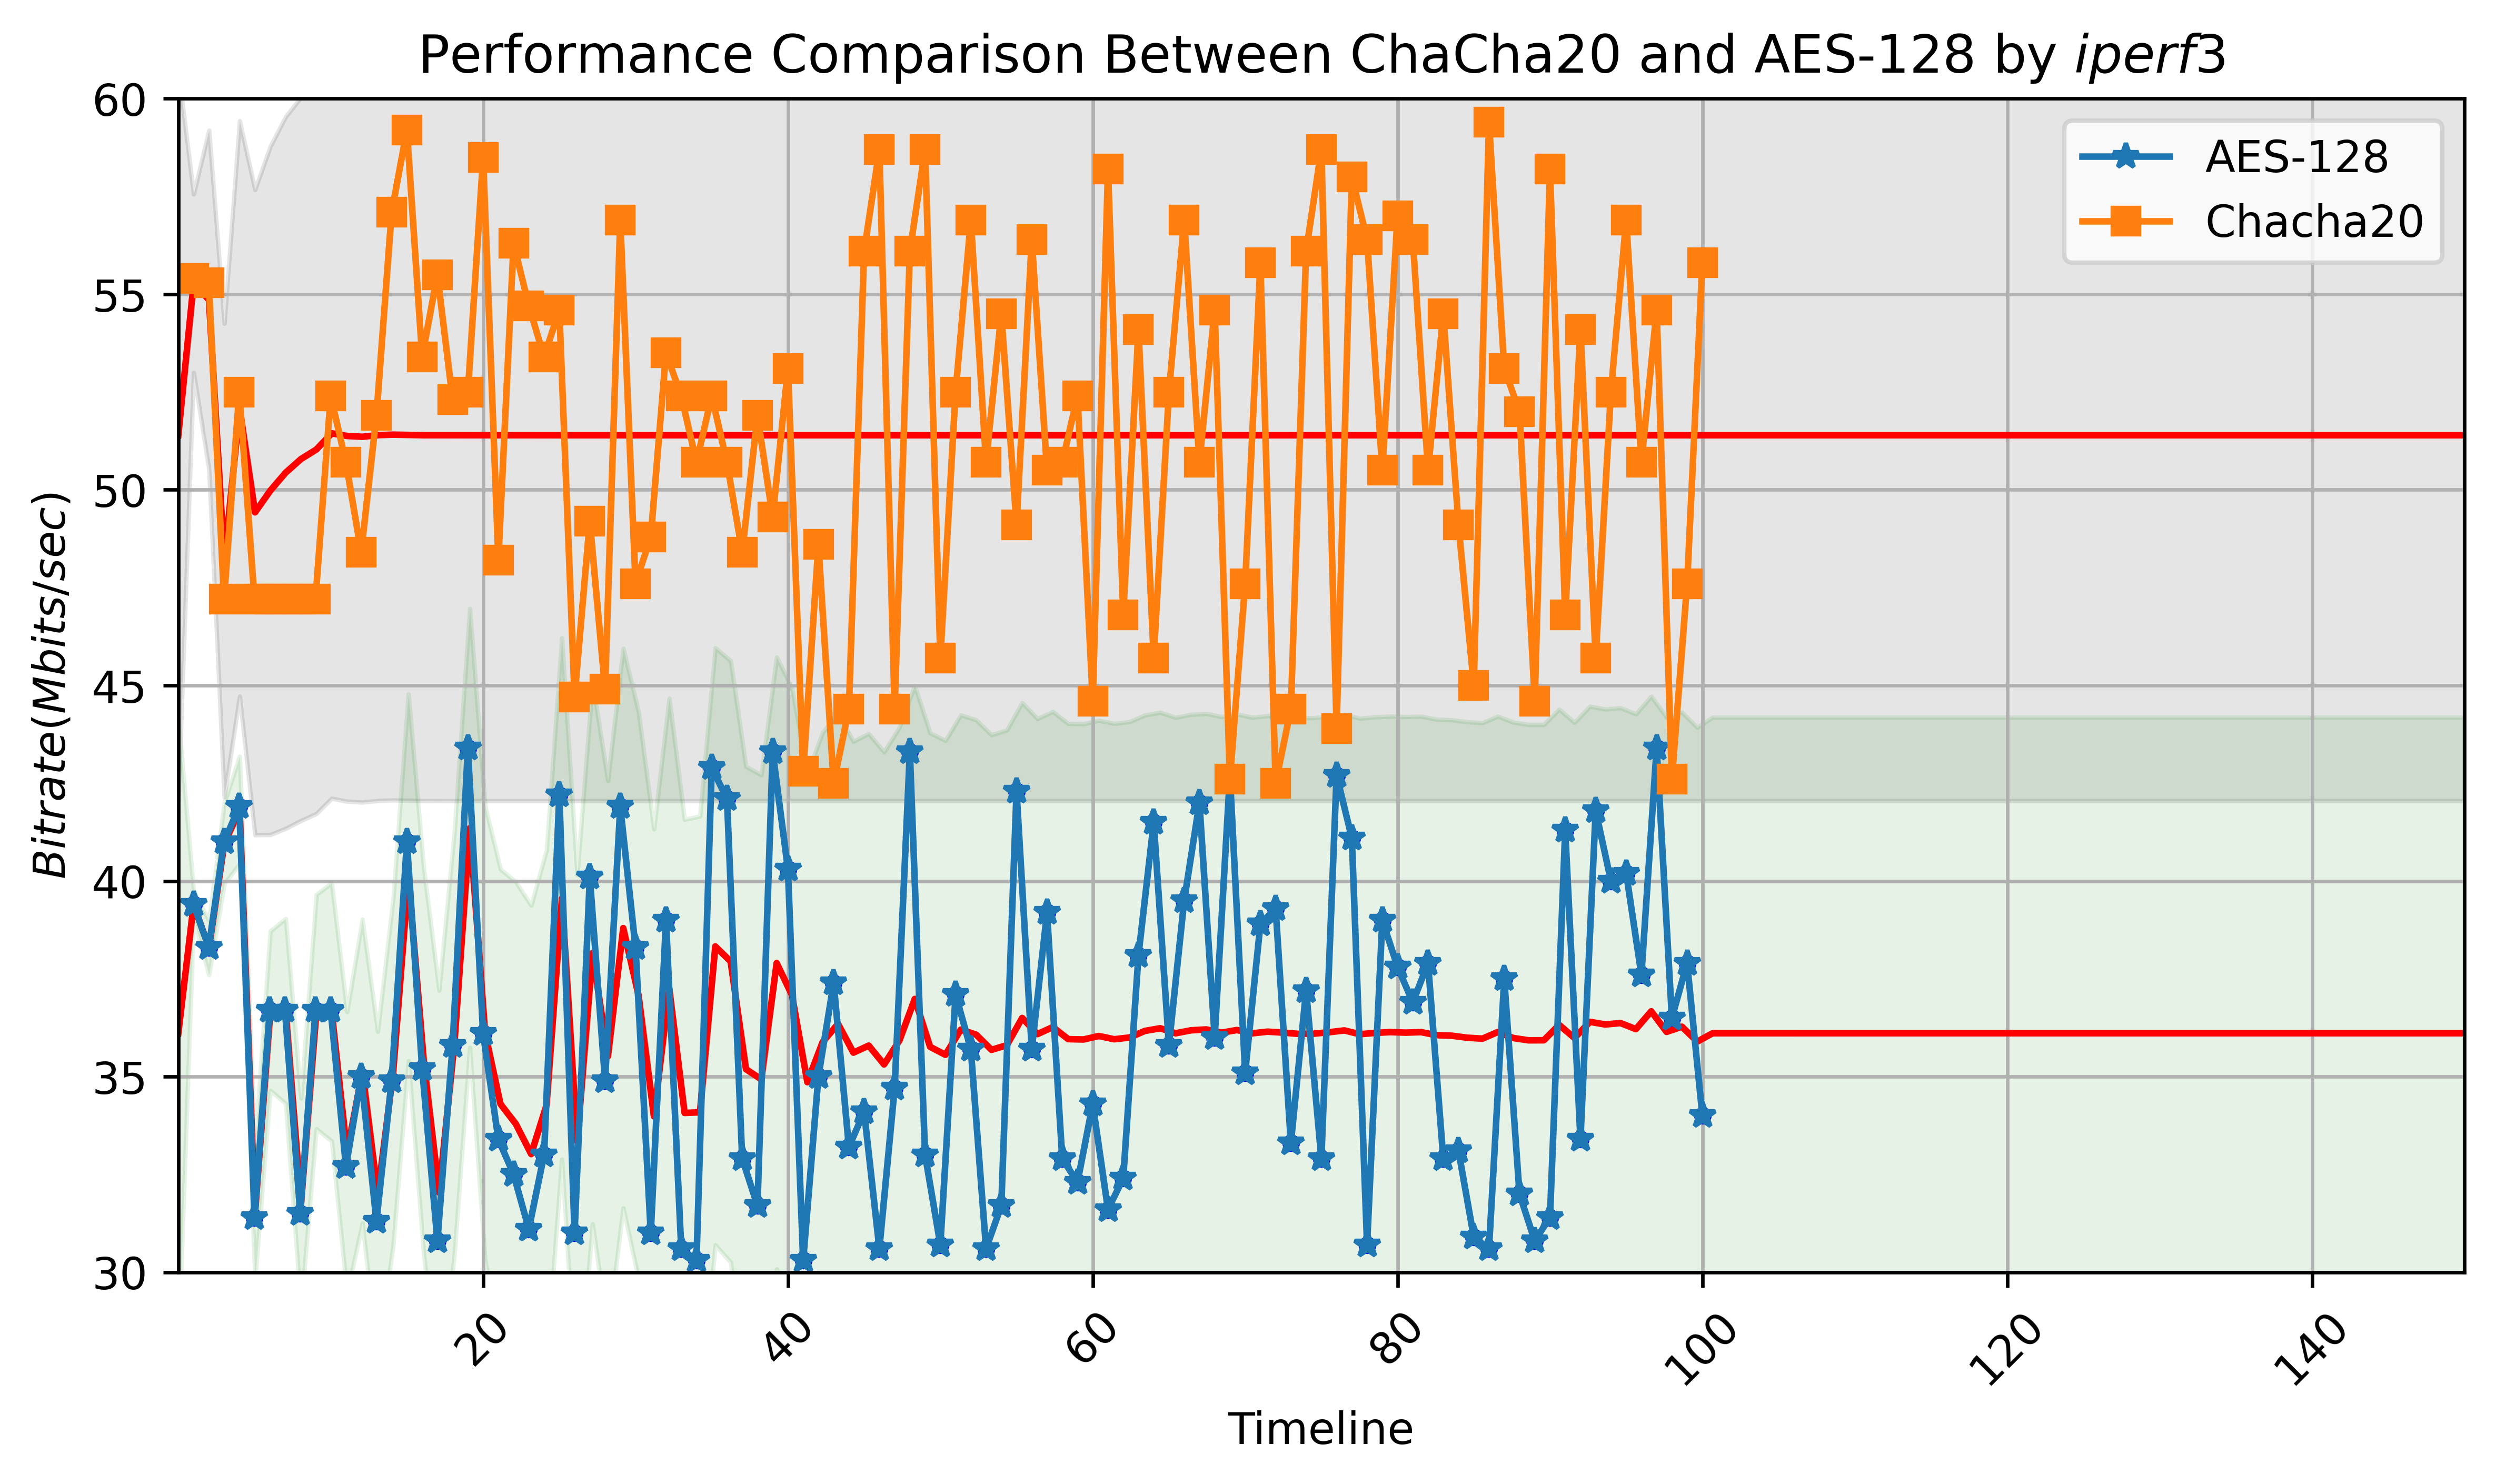
\includegraphics[width=0.8\linewidth]{fig4-2.png}
    \caption{Performance Comparison Between ChaCha20 and AES-128}
    \label{fig:4-2}
\end{figure}
The performance test comparison between ChaCha20 and AES-128, shown as Figure \ref{fig:4-2} in a embedded router system OpenWRT running on the MIPS1004Kc SOC indicates it.


% Other Partials
\backmatter

% References
\bibliography{ref/refs}  % 参考文献使用 BibTeX 编译
% \printbibliography       % 参考文献使用 BibLaTeX 编译

% Appendix
% \appendix
% \input{data/appendix-survey}       % 本科生:外文资料的调研阅读报告
% \input{data/appendix-translation}  % 本科生:外文资料的书面翻译
% \input{data/appendix}

% Acknowledgements 致谢
% \input{data/acknowledgements}

% Statement 声明
% \statement
% 将签字扫描后的声明文件 scan-statement.pdf 替换原始页面
% \statement[file=scan-statement.pdf]
% 本科生编译生成的声明页默认不加页脚,插入扫描版时再补上;
% 研究生编译生成时有页眉页脚,插入扫描版时不再重复。
% 也可以手动控制是否加页眉页脚
% \statement[page-style=empty]
% \statement[file=scan-statement.pdf, page-style=plain]

% resume
% \input{data/resume}

% Comments
% \input{data/comments}

% resolution 答辩委员会决议书
% \input{data/resolution}

% Add other files
% \record{file=scan-record.pdf}

\end{document}
